\documentclass[twoside]{book}

% Packages required by doxygen
\usepackage{fixltx2e}
\usepackage{calc}
\usepackage{doxygen}
\usepackage[export]{adjustbox} % also loads graphicx
\usepackage{graphicx}
\usepackage[utf8]{inputenc}
\usepackage{makeidx}
\usepackage{multicol}
\usepackage{multirow}
\PassOptionsToPackage{warn}{textcomp}
\usepackage{textcomp}
\usepackage[nointegrals]{wasysym}
\usepackage[table]{xcolor}

% Font selection
\usepackage[T1]{fontenc}
\usepackage[scaled=.90]{helvet}
\usepackage{courier}
\usepackage{amssymb}
\usepackage{sectsty}
\renewcommand{\familydefault}{\sfdefault}
\allsectionsfont{%
  \fontseries{bc}\selectfont%
  \color{darkgray}%
}
\renewcommand{\DoxyLabelFont}{%
  \fontseries{bc}\selectfont%
  \color{darkgray}%
}
\newcommand{\+}{\discretionary{\mbox{\scriptsize$\hookleftarrow$}}{}{}}

% Page & text layout
\usepackage{geometry}
\geometry{%
  a4paper,%
  top=2.5cm,%
  bottom=2.5cm,%
  left=2.5cm,%
  right=2.5cm%
}
\tolerance=750
\hfuzz=15pt
\hbadness=750
\setlength{\emergencystretch}{15pt}
\setlength{\parindent}{0cm}
\setlength{\parskip}{3ex plus 2ex minus 2ex}
\makeatletter
\renewcommand{\paragraph}{%
  \@startsection{paragraph}{4}{0ex}{-1.0ex}{1.0ex}{%
    \normalfont\normalsize\bfseries\SS@parafont%
  }%
}
\renewcommand{\subparagraph}{%
  \@startsection{subparagraph}{5}{0ex}{-1.0ex}{1.0ex}{%
    \normalfont\normalsize\bfseries\SS@subparafont%
  }%
}
\makeatother

% Headers & footers
\usepackage{fancyhdr}
\pagestyle{fancyplain}
\fancyhead[LE]{\fancyplain{}{\bfseries\thepage}}
\fancyhead[CE]{\fancyplain{}{}}
\fancyhead[RE]{\fancyplain{}{\bfseries\leftmark}}
\fancyhead[LO]{\fancyplain{}{\bfseries\rightmark}}
\fancyhead[CO]{\fancyplain{}{}}
\fancyhead[RO]{\fancyplain{}{\bfseries\thepage}}
\fancyfoot[LE]{\fancyplain{}{}}
\fancyfoot[CE]{\fancyplain{}{}}
\fancyfoot[RE]{\fancyplain{}{\bfseries\scriptsize Generated by Doxygen }}
\fancyfoot[LO]{\fancyplain{}{\bfseries\scriptsize Generated by Doxygen }}
\fancyfoot[CO]{\fancyplain{}{}}
\fancyfoot[RO]{\fancyplain{}{}}
\renewcommand{\footrulewidth}{0.4pt}
\renewcommand{\chaptermark}[1]{%
  \markboth{#1}{}%
}
\renewcommand{\sectionmark}[1]{%
  \markright{\thesection\ #1}%
}

% Indices & bibliography
\usepackage{natbib}
\usepackage[titles]{tocloft}
\setcounter{tocdepth}{3}
\setcounter{secnumdepth}{5}
\makeindex

% Hyperlinks (required, but should be loaded last)
\usepackage{ifpdf}
\ifpdf
  \usepackage[pdftex,pagebackref=true]{hyperref}
\else
  \usepackage[ps2pdf,pagebackref=true]{hyperref}
\fi
\hypersetup{%
  colorlinks=true,%
  linkcolor=blue,%
  citecolor=blue,%
  unicode%
}

% Custom commands
\newcommand{\clearemptydoublepage}{%
  \newpage{\pagestyle{empty}\cleardoublepage}%
}

\usepackage{caption}
\captionsetup{labelsep=space,justification=centering,font={bf},singlelinecheck=off,skip=4pt,position=top}

%===== C O N T E N T S =====

\begin{document}

% Titlepage & ToC
\hypersetup{pageanchor=false,
             bookmarksnumbered=true,
             pdfencoding=unicode
            }
\pagenumbering{alph}
\begin{titlepage}
\vspace*{7cm}
\begin{center}%
{\Large My Project }\\
\vspace*{1cm}
{\large Generated by Doxygen 1.8.13}\\
\end{center}
\end{titlepage}
\clearemptydoublepage
\pagenumbering{roman}
\tableofcontents
\clearemptydoublepage
\pagenumbering{arabic}
\hypersetup{pageanchor=true}

%--- Begin generated contents ---
\chapter{Namespace Index}
\section{Namespace List}
Here is a list of all documented namespaces with brief descriptions\+:\begin{DoxyCompactList}
\item\contentsline{section}{\hyperlink{namespace_global___planning}{Global\+\_\+\+Planning} \\*Namespace for global plannning mission }{\pageref{namespace_global___planning}}{}
\end{DoxyCompactList}

\chapter{Class Index}
\section{Class List}
Here are the classes, structs, unions and interfaces with brief descriptions\+:\begin{DoxyCompactList}
\item\contentsline{section}{\hyperlink{class_smoother}{Smoother} }{\pageref{class_smoother}}{}
\item\contentsline{section}{\hyperlink{class_global___planning_1_1_track_unit}{Global\+\_\+\+Planning\+::\+Track\+Unit} \\*Burger Tracking Control Unit }{\pageref{class_global___planning_1_1_track_unit}}{}
\end{DoxyCompactList}

\chapter{File Index}
\section{File List}
Here is a list of all documented files with brief descriptions\+:\begin{DoxyCompactList}
\item\contentsline{section}{tracking\+\_\+burger/include/tracking\+\_\+burger/{\bfseries Smoother.\+h} }{\pageref{_smoother_8h}}{}
\item\contentsline{section}{tracking\+\_\+burger/include/tracking\+\_\+burger/\hyperlink{_track_unit_8h}{Track\+Unit.\+h} }{\pageref{_track_unit_8h}}{}
\end{DoxyCompactList}

\chapter{Namespace Documentation}
\hypertarget{namespace_global___planning}{}\section{Global\+\_\+\+Planning Namespace Reference}
\label{namespace_global___planning}\index{Global\+\_\+\+Planning@{Global\+\_\+\+Planning}}


namespace for global plannning mission  


\subsection*{Classes}
\begin{DoxyCompactItemize}
\item 
class \hyperlink{class_global___planning_1_1_track_unit}{Track\+Unit}
\begin{DoxyCompactList}\small\item\em Burger Tracking Control Unit. \end{DoxyCompactList}\end{DoxyCompactItemize}


\subsection{Detailed Description}
namespace for global plannning mission 
\chapter{Class Documentation}
\hypertarget{class_smoother}{}\section{Smoother Class Reference}
\label{class_smoother}\index{Smoother@{Smoother}}


The documentation for this class was generated from the following file\+:\begin{DoxyCompactItemize}
\item 
tracking\+\_\+burger/include/tracking\+\_\+burger/Smoother.\+h\end{DoxyCompactItemize}

\hypertarget{class_global___planning_1_1_track_unit}{}\section{Global\+\_\+\+Planning\+:\+:Track\+Unit Class Reference}
\label{class_global___planning_1_1_track_unit}\index{Global\+\_\+\+Planning\+::\+Track\+Unit@{Global\+\_\+\+Planning\+::\+Track\+Unit}}


Burger Tracking Control Unit.  




{\ttfamily \#include $<$Track\+Unit.\+h$>$}

\subsection*{Public Types}
\begin{DoxyCompactItemize}
\item 
\mbox{\Hypertarget{class_global___planning_1_1_track_unit_a1e4cadd188e647288b21578bd59d624a}\label{class_global___planning_1_1_track_unit_a1e4cadd188e647288b21578bd59d624a}} 
typedef std\+::shared\+\_\+ptr$<$ \hyperlink{class_global___planning_1_1_track_unit}{Track\+Unit} $\ast$ $>$ \hyperlink{class_global___planning_1_1_track_unit_a1e4cadd188e647288b21578bd59d624a}{Ptr}
\begin{DoxyCompactList}\small\item\em shared pointer for \hyperlink{class_global___planning_1_1_track_unit}{Track\+Unit} $\ast$ We recommand to use pointer rather than a class instance. \end{DoxyCompactList}\end{DoxyCompactItemize}
\subsection*{Public Member Functions}
\begin{DoxyCompactItemize}
\item 
\mbox{\Hypertarget{class_global___planning_1_1_track_unit_af9ac69b18f983ad888a8594210ebf733}\label{class_global___planning_1_1_track_unit_af9ac69b18f983ad888a8594210ebf733}} 
\hyperlink{class_global___planning_1_1_track_unit_af9ac69b18f983ad888a8594210ebf733}{Track\+Unit} ()
\begin{DoxyCompactList}\small\item\em Construct a new Track Unit object To initialize pub\+\_\+topic, \+\_\+frame\+\_\+id\+\_\+burger, \+\_\+frame\+\_\+id\+\_\+odom, forward looking distance. \end{DoxyCompactList}\item 
\mbox{\Hypertarget{class_global___planning_1_1_track_unit_a49ac9f7d9c6d7e505bcc398ac575fa22}\label{class_global___planning_1_1_track_unit_a49ac9f7d9c6d7e505bcc398ac575fa22}} 
\hyperlink{class_global___planning_1_1_track_unit_a49ac9f7d9c6d7e505bcc398ac575fa22}{$\sim$\+Track\+Unit} ()
\begin{DoxyCompactList}\small\item\em Destroy the Track Unit object No thing to do. \end{DoxyCompactList}\item 
void \hyperlink{class_global___planning_1_1_track_unit_ae00c18addf83cc57a0ddfead96d53113}{set\+\_\+pub\+\_\+topic} (const string topic)
\begin{DoxyCompactList}\small\item\em Set the pub topic object Topic name would not be influenced by namespace defined by. \end{DoxyCompactList}\item 
void \hyperlink{class_global___planning_1_1_track_unit_a246c274d23f5e739f35720662b715feb}{set\+\_\+frame\+\_\+id\+\_\+burger} (const string burger)
\begin{DoxyCompactList}\small\item\em Set the frame id for burger object You should set frame id rightly. It\textquotesingle{}s \char`\"{}base\+\_\+footprint\char`\"{} most of the time. \char`\"{}turtlebot3\char`\"{} as default. \end{DoxyCompactList}\item 
void \hyperlink{class_global___planning_1_1_track_unit_a4a59723c0ffef932d43b837f19ac5f76}{set\+\_\+frame\+\_\+id\+\_\+odom} (const string odom)
\begin{DoxyCompactList}\small\item\em Set the frame id odom object You should set frame id rightly. It\textquotesingle{}s \char`\"{}map\char`\"{} most of the time. \end{DoxyCompactList}\item 
void \hyperlink{class_global___planning_1_1_track_unit_ae34bc618e5a33012f26d986883b6ead3}{set\+\_\+fw\+\_\+lk\+\_\+distance} (const double new\+\_\+dist)
\begin{DoxyCompactList}\small\item\em Set forward looking distance Forward looking distance refers to the length from furthest traking point to current postion. A higher value should be passed when the mechine is expected to trace path smoothly. However, a great value would make mechine ingore some shape point of the path. \end{DoxyCompactList}\item 
void \hyperlink{class_global___planning_1_1_track_unit_ae78e6a634662dce0f8c48a0caba8a38d}{pub\+\_\+control} (const nav\+\_\+msgs\+::\+Path \&path, const geometry\+\_\+msgs\+::\+Pose \&cur\+\_\+pos) const
\begin{DoxyCompactList}\small\item\em publish control command to burger One invoking means one publishing without spin\+Once. It can be used in while-\/loop or callback function. \end{DoxyCompactList}\item 
int \hyperlink{class_global___planning_1_1_track_unit_af206846d5a6ddbef34e23341a9dcf5d1}{get\+\_\+closest\+\_\+point\+\_\+id} (const nav\+\_\+msgs\+::\+Path \&path, const geometry\+\_\+msgs\+::\+Pose \&cur\+\_\+pos) const
\begin{DoxyCompactList}\small\item\em Get the closest point index of the path This function is for special using. \end{DoxyCompactList}\item 
int \hyperlink{class_global___planning_1_1_track_unit_ab55bd7b7b30500844bad389101ca9a0c}{get\+\_\+track\+\_\+point\+\_\+id} (const nav\+\_\+msgs\+::\+Path \&path, const geometry\+\_\+msgs\+::\+Pose \&cur\+\_\+pos) const
\begin{DoxyCompactList}\small\item\em Get the track point index of the path This function is for special using. \end{DoxyCompactList}\end{DoxyCompactItemize}


\subsection{Detailed Description}
Burger Tracking Control Unit. 



\subsection{Member Function Documentation}
\mbox{\Hypertarget{class_global___planning_1_1_track_unit_af206846d5a6ddbef34e23341a9dcf5d1}\label{class_global___planning_1_1_track_unit_af206846d5a6ddbef34e23341a9dcf5d1}} 
\index{Global\+\_\+\+Planning\+::\+Track\+Unit@{Global\+\_\+\+Planning\+::\+Track\+Unit}!get\+\_\+closest\+\_\+point\+\_\+id@{get\+\_\+closest\+\_\+point\+\_\+id}}
\index{get\+\_\+closest\+\_\+point\+\_\+id@{get\+\_\+closest\+\_\+point\+\_\+id}!Global\+\_\+\+Planning\+::\+Track\+Unit@{Global\+\_\+\+Planning\+::\+Track\+Unit}}
\subsubsection{\texorpdfstring{get\+\_\+closest\+\_\+point\+\_\+id()}{get\_closest\_point\_id()}}
{\footnotesize\ttfamily int Global\+\_\+\+Planning\+::\+Track\+Unit\+::get\+\_\+closest\+\_\+point\+\_\+id (\begin{DoxyParamCaption}\item[{const nav\+\_\+msgs\+::\+Path \&}]{path,  }\item[{const geometry\+\_\+msgs\+::\+Pose \&}]{cur\+\_\+pos }\end{DoxyParamCaption}) const}



Get the closest point index of the path This function is for special using. 


\begin{DoxyParams}{Parameters}
{\em path} & is the waypoints mechine is expected to trace \\
\hline
{\em cur\+\_\+pos} & is current position (meter) \\
\hline
\end{DoxyParams}
\begin{DoxyReturn}{Returns}
int is the index of path waypoint 
\end{DoxyReturn}
\mbox{\Hypertarget{class_global___planning_1_1_track_unit_ab55bd7b7b30500844bad389101ca9a0c}\label{class_global___planning_1_1_track_unit_ab55bd7b7b30500844bad389101ca9a0c}} 
\index{Global\+\_\+\+Planning\+::\+Track\+Unit@{Global\+\_\+\+Planning\+::\+Track\+Unit}!get\+\_\+track\+\_\+point\+\_\+id@{get\+\_\+track\+\_\+point\+\_\+id}}
\index{get\+\_\+track\+\_\+point\+\_\+id@{get\+\_\+track\+\_\+point\+\_\+id}!Global\+\_\+\+Planning\+::\+Track\+Unit@{Global\+\_\+\+Planning\+::\+Track\+Unit}}
\subsubsection{\texorpdfstring{get\+\_\+track\+\_\+point\+\_\+id()}{get\_track\_point\_id()}}
{\footnotesize\ttfamily int Global\+\_\+\+Planning\+::\+Track\+Unit\+::get\+\_\+track\+\_\+point\+\_\+id (\begin{DoxyParamCaption}\item[{const nav\+\_\+msgs\+::\+Path \&}]{path,  }\item[{const geometry\+\_\+msgs\+::\+Pose \&}]{cur\+\_\+pos }\end{DoxyParamCaption}) const}



Get the track point index of the path This function is for special using. 


\begin{DoxyParams}{Parameters}
{\em path} & is the waypoints mechine is expected to trace \\
\hline
{\em cur\+\_\+pos} & is current position (meter) \\
\hline
\end{DoxyParams}
\begin{DoxyReturn}{Returns}
int is the index of path waypoint 
\end{DoxyReturn}
\mbox{\Hypertarget{class_global___planning_1_1_track_unit_ae78e6a634662dce0f8c48a0caba8a38d}\label{class_global___planning_1_1_track_unit_ae78e6a634662dce0f8c48a0caba8a38d}} 
\index{Global\+\_\+\+Planning\+::\+Track\+Unit@{Global\+\_\+\+Planning\+::\+Track\+Unit}!pub\+\_\+control@{pub\+\_\+control}}
\index{pub\+\_\+control@{pub\+\_\+control}!Global\+\_\+\+Planning\+::\+Track\+Unit@{Global\+\_\+\+Planning\+::\+Track\+Unit}}
\subsubsection{\texorpdfstring{pub\+\_\+control()}{pub\_control()}}
{\footnotesize\ttfamily void Global\+\_\+\+Planning\+::\+Track\+Unit\+::pub\+\_\+control (\begin{DoxyParamCaption}\item[{const nav\+\_\+msgs\+::\+Path \&}]{path,  }\item[{const geometry\+\_\+msgs\+::\+Pose \&}]{cur\+\_\+pos }\end{DoxyParamCaption}) const}



publish control command to burger One invoking means one publishing without spin\+Once. It can be used in while-\/loop or callback function. 


\begin{DoxyParams}{Parameters}
{\em path} & is the waypoints mechine is expected to trace \\
\hline
{\em cur\+\_\+pos} & is current position (meter) \\
\hline
\end{DoxyParams}
\mbox{\Hypertarget{class_global___planning_1_1_track_unit_a246c274d23f5e739f35720662b715feb}\label{class_global___planning_1_1_track_unit_a246c274d23f5e739f35720662b715feb}} 
\index{Global\+\_\+\+Planning\+::\+Track\+Unit@{Global\+\_\+\+Planning\+::\+Track\+Unit}!set\+\_\+frame\+\_\+id\+\_\+burger@{set\+\_\+frame\+\_\+id\+\_\+burger}}
\index{set\+\_\+frame\+\_\+id\+\_\+burger@{set\+\_\+frame\+\_\+id\+\_\+burger}!Global\+\_\+\+Planning\+::\+Track\+Unit@{Global\+\_\+\+Planning\+::\+Track\+Unit}}
\subsubsection{\texorpdfstring{set\+\_\+frame\+\_\+id\+\_\+burger()}{set\_frame\_id\_burger()}}
{\footnotesize\ttfamily void Global\+\_\+\+Planning\+::\+Track\+Unit\+::set\+\_\+frame\+\_\+id\+\_\+burger (\begin{DoxyParamCaption}\item[{const string}]{burger }\end{DoxyParamCaption})}



Set the frame id for burger object You should set frame id rightly. It\textquotesingle{}s \char`\"{}base\+\_\+footprint\char`\"{} most of the time. \char`\"{}turtlebot3\char`\"{} as default. 


\begin{DoxyParams}{Parameters}
{\em burger} & \\
\hline
\end{DoxyParams}
\mbox{\Hypertarget{class_global___planning_1_1_track_unit_a4a59723c0ffef932d43b837f19ac5f76}\label{class_global___planning_1_1_track_unit_a4a59723c0ffef932d43b837f19ac5f76}} 
\index{Global\+\_\+\+Planning\+::\+Track\+Unit@{Global\+\_\+\+Planning\+::\+Track\+Unit}!set\+\_\+frame\+\_\+id\+\_\+odom@{set\+\_\+frame\+\_\+id\+\_\+odom}}
\index{set\+\_\+frame\+\_\+id\+\_\+odom@{set\+\_\+frame\+\_\+id\+\_\+odom}!Global\+\_\+\+Planning\+::\+Track\+Unit@{Global\+\_\+\+Planning\+::\+Track\+Unit}}
\subsubsection{\texorpdfstring{set\+\_\+frame\+\_\+id\+\_\+odom()}{set\_frame\_id\_odom()}}
{\footnotesize\ttfamily void Global\+\_\+\+Planning\+::\+Track\+Unit\+::set\+\_\+frame\+\_\+id\+\_\+odom (\begin{DoxyParamCaption}\item[{const string}]{odom }\end{DoxyParamCaption})}



Set the frame id odom object You should set frame id rightly. It\textquotesingle{}s \char`\"{}map\char`\"{} most of the time. 


\begin{DoxyParams}{Parameters}
{\em odom} & \\
\hline
\end{DoxyParams}
\mbox{\Hypertarget{class_global___planning_1_1_track_unit_ae34bc618e5a33012f26d986883b6ead3}\label{class_global___planning_1_1_track_unit_ae34bc618e5a33012f26d986883b6ead3}} 
\index{Global\+\_\+\+Planning\+::\+Track\+Unit@{Global\+\_\+\+Planning\+::\+Track\+Unit}!set\+\_\+fw\+\_\+lk\+\_\+distance@{set\+\_\+fw\+\_\+lk\+\_\+distance}}
\index{set\+\_\+fw\+\_\+lk\+\_\+distance@{set\+\_\+fw\+\_\+lk\+\_\+distance}!Global\+\_\+\+Planning\+::\+Track\+Unit@{Global\+\_\+\+Planning\+::\+Track\+Unit}}
\subsubsection{\texorpdfstring{set\+\_\+fw\+\_\+lk\+\_\+distance()}{set\_fw\_lk\_distance()}}
{\footnotesize\ttfamily void Global\+\_\+\+Planning\+::\+Track\+Unit\+::set\+\_\+fw\+\_\+lk\+\_\+distance (\begin{DoxyParamCaption}\item[{const double}]{new\+\_\+dist }\end{DoxyParamCaption})}



Set forward looking distance Forward looking distance refers to the length from furthest traking point to current postion. A higher value should be passed when the mechine is expected to trace path smoothly. However, a great value would make mechine ingore some shape point of the path. 


\begin{DoxyParams}{Parameters}
{\em new\+\_\+dist} & forward looking distance (meter) -\/ 1.\+0 as default \\
\hline
\end{DoxyParams}
\mbox{\Hypertarget{class_global___planning_1_1_track_unit_ae00c18addf83cc57a0ddfead96d53113}\label{class_global___planning_1_1_track_unit_ae00c18addf83cc57a0ddfead96d53113}} 
\index{Global\+\_\+\+Planning\+::\+Track\+Unit@{Global\+\_\+\+Planning\+::\+Track\+Unit}!set\+\_\+pub\+\_\+topic@{set\+\_\+pub\+\_\+topic}}
\index{set\+\_\+pub\+\_\+topic@{set\+\_\+pub\+\_\+topic}!Global\+\_\+\+Planning\+::\+Track\+Unit@{Global\+\_\+\+Planning\+::\+Track\+Unit}}
\subsubsection{\texorpdfstring{set\+\_\+pub\+\_\+topic()}{set\_pub\_topic()}}
{\footnotesize\ttfamily void Global\+\_\+\+Planning\+::\+Track\+Unit\+::set\+\_\+pub\+\_\+topic (\begin{DoxyParamCaption}\item[{const string}]{topic }\end{DoxyParamCaption})}



Set the pub topic object Topic name would not be influenced by namespace defined by. 


\begin{DoxyParams}{Parameters}
{\em topic} & is the topic to which you want to publish infomations \\
\hline
\end{DoxyParams}


The documentation for this class was generated from the following file\+:\begin{DoxyCompactItemize}
\item 
tracking\+\_\+burger/include/tracking\+\_\+burger/\hyperlink{_track_unit_8h}{Track\+Unit.\+h}\end{DoxyCompactItemize}

\chapter{File Documentation}
\hypertarget{_track_unit_8h}{}\section{tracking\+\_\+burger/include/tracking\+\_\+burger/\+Track\+Unit.h File Reference}
\label{_track_unit_8h}\index{tracking\+\_\+burger/include/tracking\+\_\+burger/\+Track\+Unit.\+h@{tracking\+\_\+burger/include/tracking\+\_\+burger/\+Track\+Unit.\+h}}
{\ttfamily \#include \char`\"{}ros/ros.\+h\char`\"{}}\newline
{\ttfamily \#include \char`\"{}geometry\+\_\+msgs/\+Twist.\+h\char`\"{}}\newline
{\ttfamily \#include \char`\"{}nav\+\_\+msgs/\+Path.\+h\char`\"{}}\newline
{\ttfamily \#include \char`\"{}geometry\+\_\+msgs/\+Pose.\+h\char`\"{}}\newline
{\ttfamily \#include $<$memory$>$}\newline
{\ttfamily \#include $<$string$>$}\newline
Include dependency graph for Track\+Unit.\+h\+:
\nopagebreak
\begin{figure}[H]
\begin{center}
\leavevmode
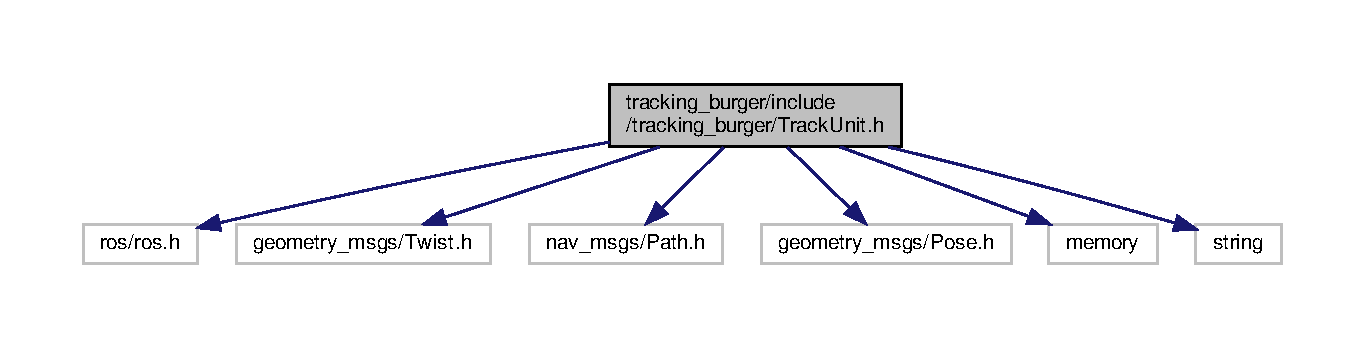
\includegraphics[width=350pt]{_track_unit_8h__incl}
\end{center}
\end{figure}
\subsection*{Classes}
\begin{DoxyCompactItemize}
\item 
class \hyperlink{class_global___planning_1_1_track_unit}{Global\+\_\+\+Planning\+::\+Track\+Unit}
\begin{DoxyCompactList}\small\item\em Burger Tracking Control Unit. \end{DoxyCompactList}\end{DoxyCompactItemize}
\subsection*{Namespaces}
\begin{DoxyCompactItemize}
\item 
 \hyperlink{namespace_global___planning}{Global\+\_\+\+Planning}
\begin{DoxyCompactList}\small\item\em namespace for global plannning mission \end{DoxyCompactList}\end{DoxyCompactItemize}


\subsection{Detailed Description}
\begin{DoxyAuthor}{Author}
Vinson Sheep (\href{mailto:775014077@qq.com}{\tt 775014077@qq.\+com}) 
\end{DoxyAuthor}
\begin{DoxyVersion}{Version}
0.\+1 
\end{DoxyVersion}
\begin{DoxyDate}{Date}
2021-\/04-\/28
\end{DoxyDate}
\begin{DoxyCopyright}{Copyright}
Copyright (c) 2021 
\end{DoxyCopyright}

%--- End generated contents ---

% Index
\backmatter
\newpage
\phantomsection
\clearemptydoublepage
\addcontentsline{toc}{chapter}{Index}
\printindex

\end{document}
